\documentclass[12pt]{article}

\usepackage{geometry}
\usepackage{amsmath}
\usepackage{tikz}
\usepackage{paralist}
\usepackage{enumerate}
\usepackage{amsfonts}
\usepackage{verbatim}
\usepackage{multirow}
\usepackage{subcaption}



\newcommand{\ds}{\displaystyle}
\newcommand{\ra}{\rightarrow}
\newcommand{\Ra}{\Rightarrow}
\newcommand{\la}{\leftarrow}
\newcommand{\La}{\Leftarrow}

\newtheorem{thm}{Theorem}%[section]
\newtheorem{lem}{Lemma}%[theorem]
\newtheorem{prop}{Proposition}%[theorem]
\newtheorem{cor}{Corollary}%[theorem]
\newtheorem{defn}{Definition}



\title{MA585 Final Project: Modeling Baseball Teams' Yearly Winning Percentage With Time Series Models}
\author{Samuel Greeman}
\date{Due April 29, 2021}


\begin{document}
\maketitle 



\setdefaultleftmargin{0pt}{}{}{}{}{}

\section{Introduction/Summary and Data Modification}\label{sec:intro}
The goal today is to find out if team success in sports year-by-year can be accurately modeled by a time series model. To accomplish this, we created a dataset [1] of the Cincinnati Reds' yearly win totals from 1947-2019. The reason we chose to start in 1947 is that 1947 was the start of racial integration in Major League Baseball. We did not include the 2020 season as it was shortened by over 100 games due to COVID-19. Some modifications had to be made to this data to make it a comparable dataset year by year. The first issue was normalizing the number of games played per season. From 1947-1961, there were 154 scheduled games for each team, and from 1962-2019, the number increased to 162. However, in 1981, 1994, and 1995, labor issues led to strikes from players and ultimately, fewer games were played in those years. To normalize all of these discrepancies, I instead used winning percentage as the key variable instead of total wins, as winning percentage is on the same scale no matter how many games are played. Typically, for baseball teams, winning percentages fall in the range of 0.400 to 0.600, with the lowest all time being 0.250 and the highest being 0.716. After comparisons using ARIMA(0, 1, 1), exponential smoothing, and Holt-Winters method as our 3 models, we decided that the Holt-Winters method is most effective at modeling the trends in teams' year-by-year winning percentage. With the data read in, let's look at how we got to this conclusion, starting by seeing how it looks as a time series.\\

\section{Visual Analysis}\label{sec:chapter}
\begin{figure}[h!]
\centering
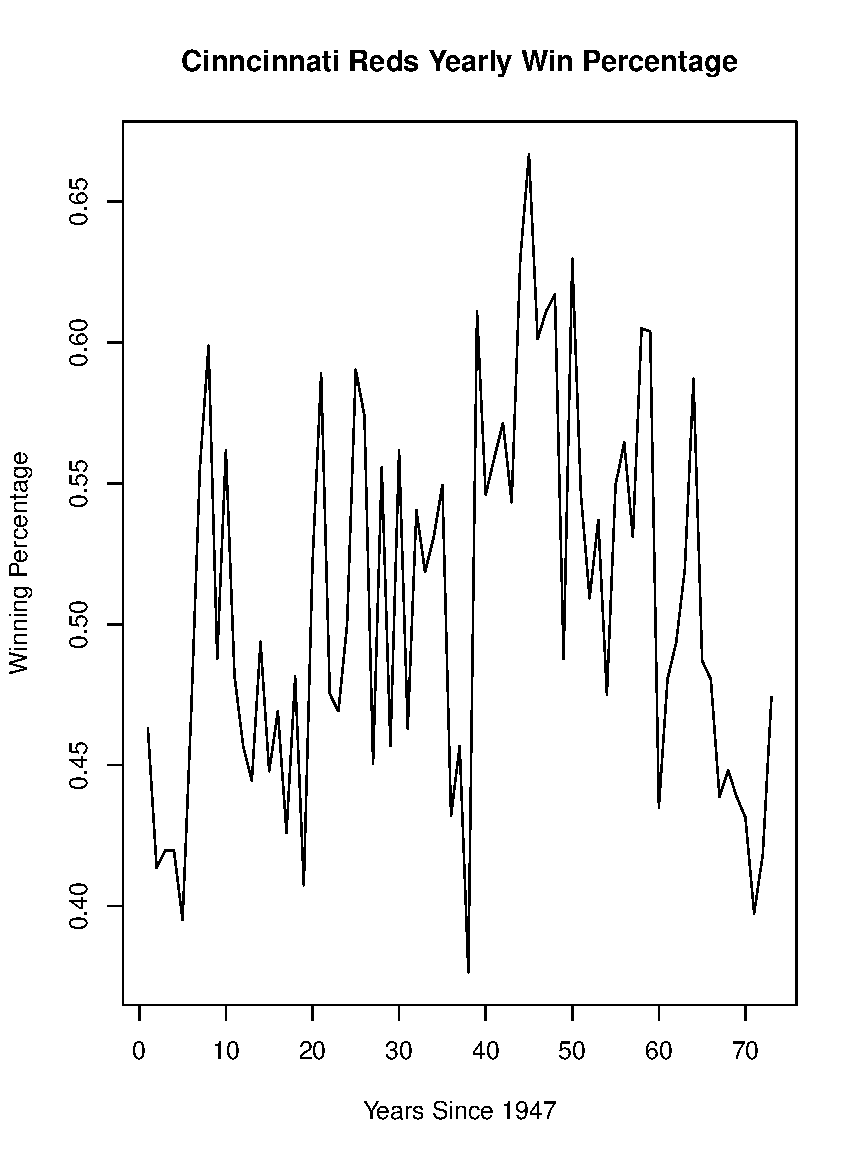
\includegraphics[scale=0.6]{Reds Win Pct.pdf}
\caption{Plot of Time Series Data}
\label{fig:Figure 1}
\end{figure} 
Looking at figure 1, we see that the winning percentage, as expected fluctuates between 0.400 and 0.650. We can calculate the average winning percentage over this 73 year span, and get 0.507. This tells us that while there were some ups and downs, the Reds were a fairly average team over this 73 year span, which is good since it means that this analysis will be fairly representative of MLB teams as a whole. One problem we can see is that the mean doesn't appear to be constant over time. There are two ways we decided to eliminate this trend, which we will learn about next. \\

\section{Differencing}\label{sec:chapter}
The first way we can try to eliminate this trend is by differencing. Differencing is effective at eliminating a trend that renders a set of data as nonstationary, and here, we will use the order of differencing, k, to be 1. After differencing, our data looks like this:\\
\begin{figure}[h!]
\centering
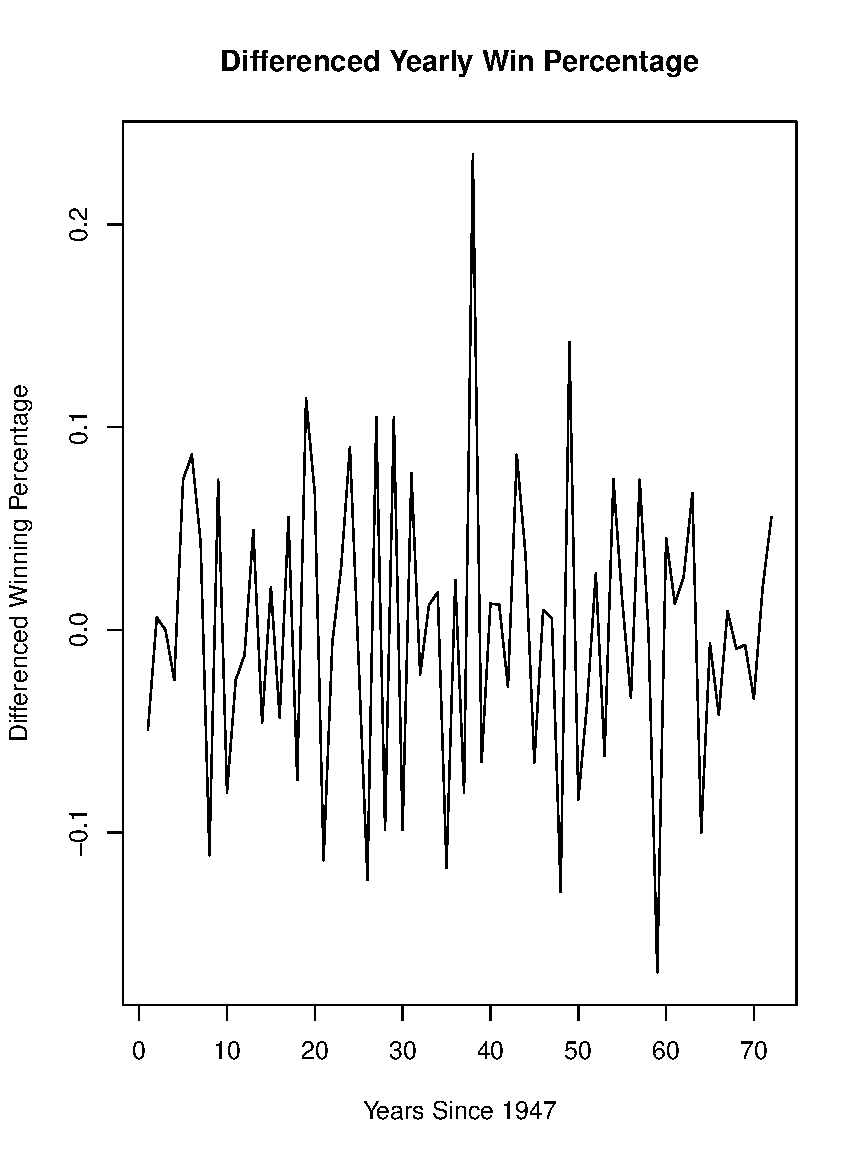
\includegraphics[scale=0.6]{Differenced Win.pdf}
\caption{Plot of Differenced Time Series Data}
\label{fig:Figure 2}
\end{figure}\\
Now we can see that the mean stays relatively constant over time. The variance looks fairly constant over time as well, so in our next section, we can try to create an ARIMA model with a difference order of 1. Before that, let's address our other method of trend elimination.\\

\section{Exponential Smoothing}\label{sec:chapter}
Exponential smoothing works best when there are sharp peaks and valleys in time series data, and it helps to smooth them out, as the name suggests. We decided to go with a large smoothing parameter of \(\lambda = 0.6\), as the peaks and valleys are pretty extreme. The plot of our fitted exponentially smoothed data looks like this:\\
\begin{figure}[h!]
\centering
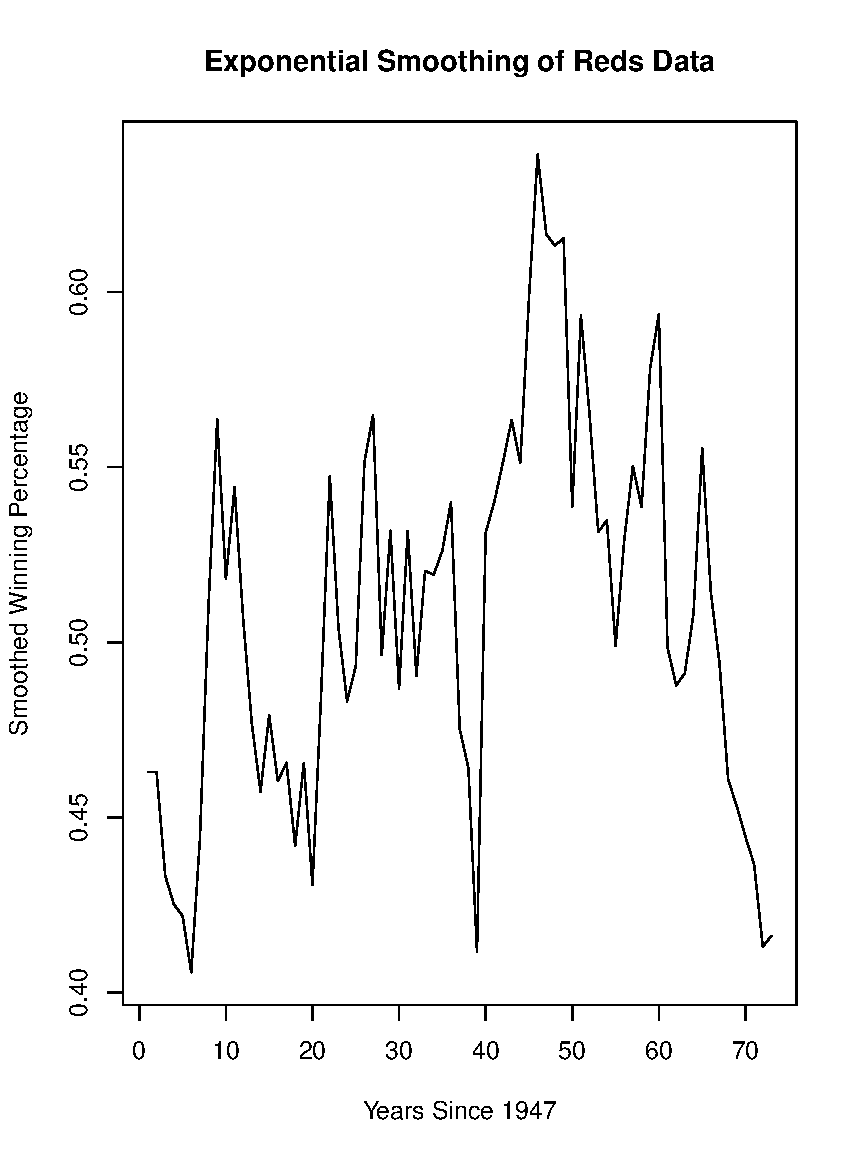
\includegraphics[scale=0.6]{ES plot.pdf}
\caption{Plot of Exponentially Smoothed Time Series Data (\(\lambda = 0.6\))}
\label{fig:Figure 3}
\end{figure}\\
While we can see some evidence of non-constant mean, this at least helped the problem of extremely erratic data from year to year. We can see that the slow rise ending at \(x = 45\) is still there, but is much less than it was originally. With these methods complete, we can now try to create effective models.\\

\section{Model Creation}\label{sec:chapter}
Since the exponential smoothing actually creates a model for our data, we can leave it alone until we test it. When we looked at the differenced data, we saw that it eliminated a trend and made it stationary, and a Dickey-Fuller test on both datasets backs up this claim. For the original dataset, the Dickey-Fuller test gave us a test statistic of \(-2.242\) and a p-value of \(0.4768\), indicating that we fail to reject the null hypothesis of nonstationarity. Running the same test on our differenced data, we get a test statistic of \(-5.362\) and a p-value smaller than \(0.01\), meaning we reject the null hypothesis of nonstationarity for the alternative hypothesis of stationarity. This means that when we search for an ARIMA model, our d value for ARIMA(p, d, q) should be 1 to indicate differencing of order 1. To find possible values of p and q, let's look at the ACF and PACF plots:\\
\begin{figure}[h]
\begin{subfigure}{0.5\textwidth}
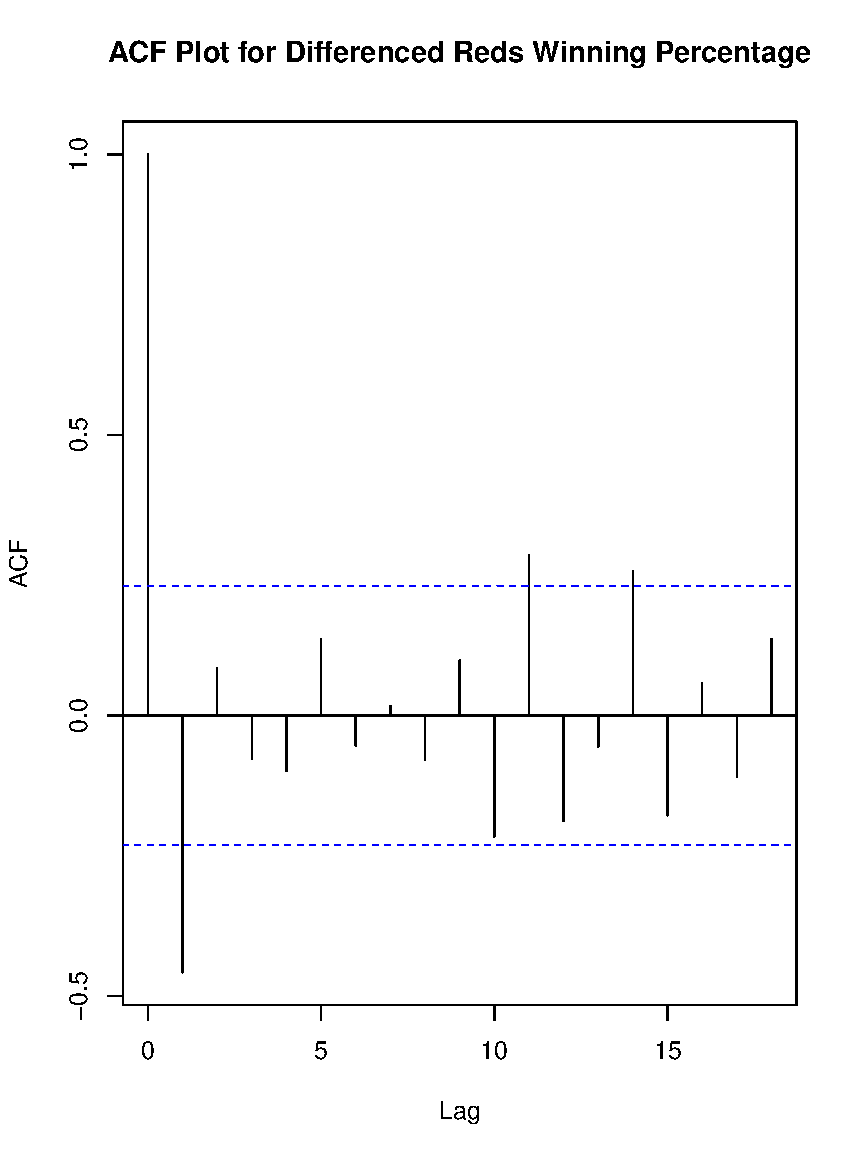
\includegraphics[width=0.9\linewidth, height=9cm]{dacf.pdf} 
\caption{ACF Plot of Differenced Data}
\label{fig:subim1}
\end{subfigure}
\begin{subfigure}{0.5\textwidth}
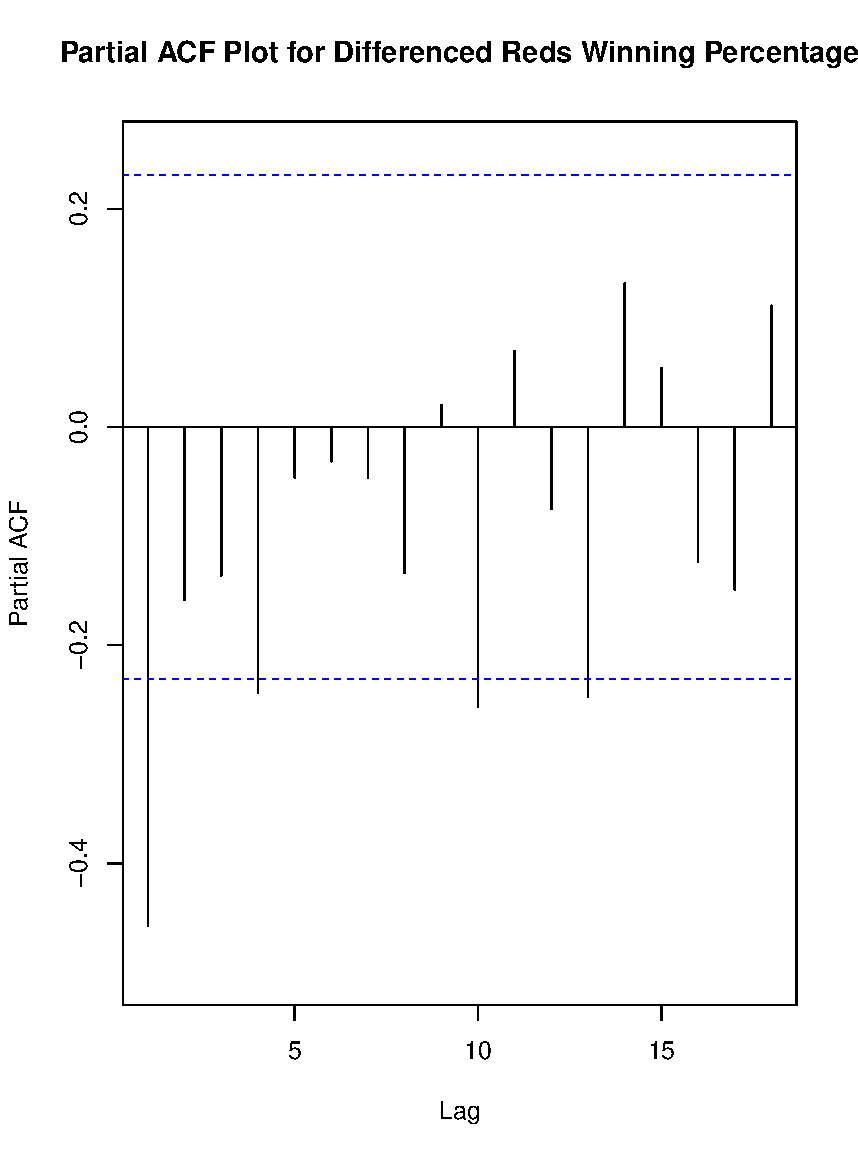
\includegraphics[width=0.9\linewidth, height=9cm]{dpacf.pdf}
\caption{PACF Plot of Differenced Data}
\label{fig:subim2}
\end{subfigure}
\caption{PACF and ACF Plots for Differenced Data}
\label{fig:Figure 4}
\end{figure}\\
Immediately, we see from figure 4 that we likely don't need an AR term, rather we need an MA term in our ARIMA model. Not only are our ACF and PACF values at lag 1 the same, but the ACF cuts off after lag 1, and the PACF decays to 0, both of which indicate \(q = 1\). When we compare AIC for other models, such as ARIMA(2, 1, 0), and ARIMA(1, 1, 1) and other low order ARIMA models with \(d = 1\), we see that ARIMA(0, 1, 1) has the lowest AIC at \(-193.94\), and the parameters can either be found using R, or by hand. We can see that the ACF and PACF at lag 1 is around \(-0.46\), and ACF at lag 1 for an MA(1) process is \(\frac{\theta}{1 + \theta^2}\) and if we set that relationship equal to \(-0.46\), we get \(\theta = -0.661\). Using R, we get a similar value of \(\theta = -0.6604\). We will use R's value as it is likely more precise than our estimation.\\

\section{Model Testing}\label{sec:chapter}
Now that we have 2 (and a third to be introduced soon) models, we can test their accuracy using forecasts based on our actual data. In order to this, we take the first 66 years of our dataset and use them as our training data, and we will test the models we created on the remaining 7 years and see how close they are. I mentioned a third model, and that model is Holt-Winters. We mentioned in the exponential smoothing section that while the smoothing did an adequate job of smoothing the peaks and valleys in our dataset, there still seemed to be nonstationarirty in regard to the non-constant mean. Holt-Winters method is effective at forecasting the trend of the mean in addition to using exponential smoothing, so the Holt-Winters method will be our 3rd and final model. After training our models and testing them, we get these results in table 1 that tell us the forecasted winning percentage for the final 7 years in addition to the 95 percent forecast interval for the values.\\
\begin{table}[h]
\begin{center}
\begin{tabular}{ |c|c|c|c|c| } 
 \hline
 \textbf{Year} & \textbf{Actual} & \textbf{Holt-Winters} & \textbf{ARIMA(0, 1, 1)} & \textbf{Exp. Smoothing} \\
 \hline
 2013 & 0.556 & 0.489, (0.347, 0.632) & 0.510, (0.388, 0.633) & 0.494, (0.367, 0.621)\\
 \hline
 2014 & 0.469 & 0.485, (0.315, 0.654) & 0.510, (0.384, 0.637) & 0.494, (0.346, 0.642)\\ 
 \hline
 2015 & 0.395 & 0.480, (0.281, 0.678) & 0.510, (0.380, 0.641) & 0.494, (0.327, 0.661)\\ 
 \hline
 2016 & 0.420 & 0.475, (0.246, 0.703) & 0.510, (0.376, 0.645) & 0.494, (0.311, 0.677)\\ 
 \hline
 2017 & 0.420 & 0.470, (0.209, 0.731) & 0.510, (0.372, 0.649) & 0.494, (0.296, 0.693)\\ 
 \hline
 2018 & 0.414 & 0.465, (0.170, 0.759) & 0.510, (0.368, 0.653) & 0.494, (0.281, 0.707)\\ 
 \hline
 2019 & 0.463 & 0.460, (0.130, 0.790) & 0.510, (0.365, 0.657) & 0.494, (0.268, 0.720)\\ 
 \hline
\end{tabular}
\caption{Forecasted Win Percentages from our 3 models}
\label{table:Table 1}
\end{center}
\end{table}\\
The key things to note are that the Holt-Winters method is the only model that uses a nonconstant mean, which is important in this case because we found that the mean for data like this is nonconstant. The ARIMA forecast uses a constant mean after differencing, and the exponential smoothing forecast uses a constant mean from the start. Figure 5 shows how Holt-Winters forecasts the trend of the mean, while the other 2 models simply increase the size of the interval each year while keeping their forecast constant:\\
\begin{figure}[h]
\begin{subfigure}{0.32\textwidth}
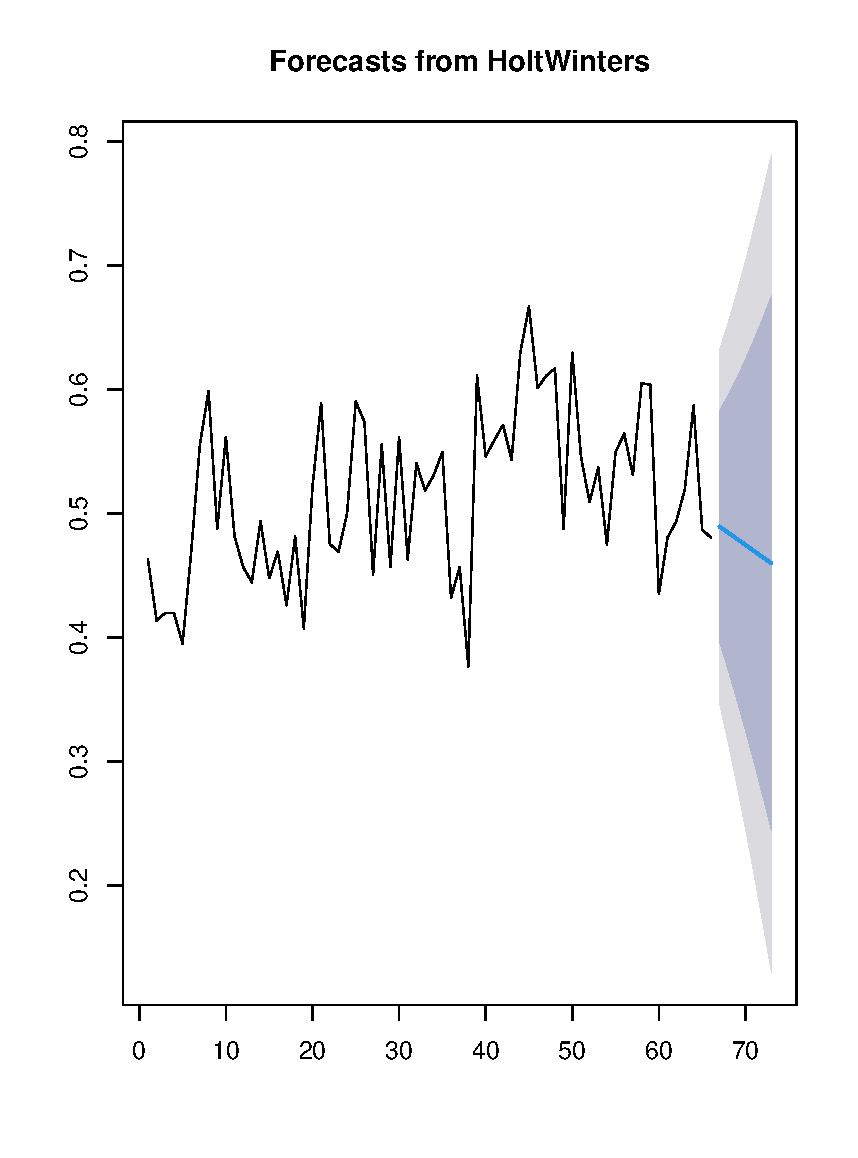
\includegraphics[width=0.9\linewidth, height=9cm]{hw fore.pdf} 
\caption{Holt-Winters Forecast}
\label{fig:subim1}
\end{subfigure}
\begin{subfigure}{0.32\textwidth}
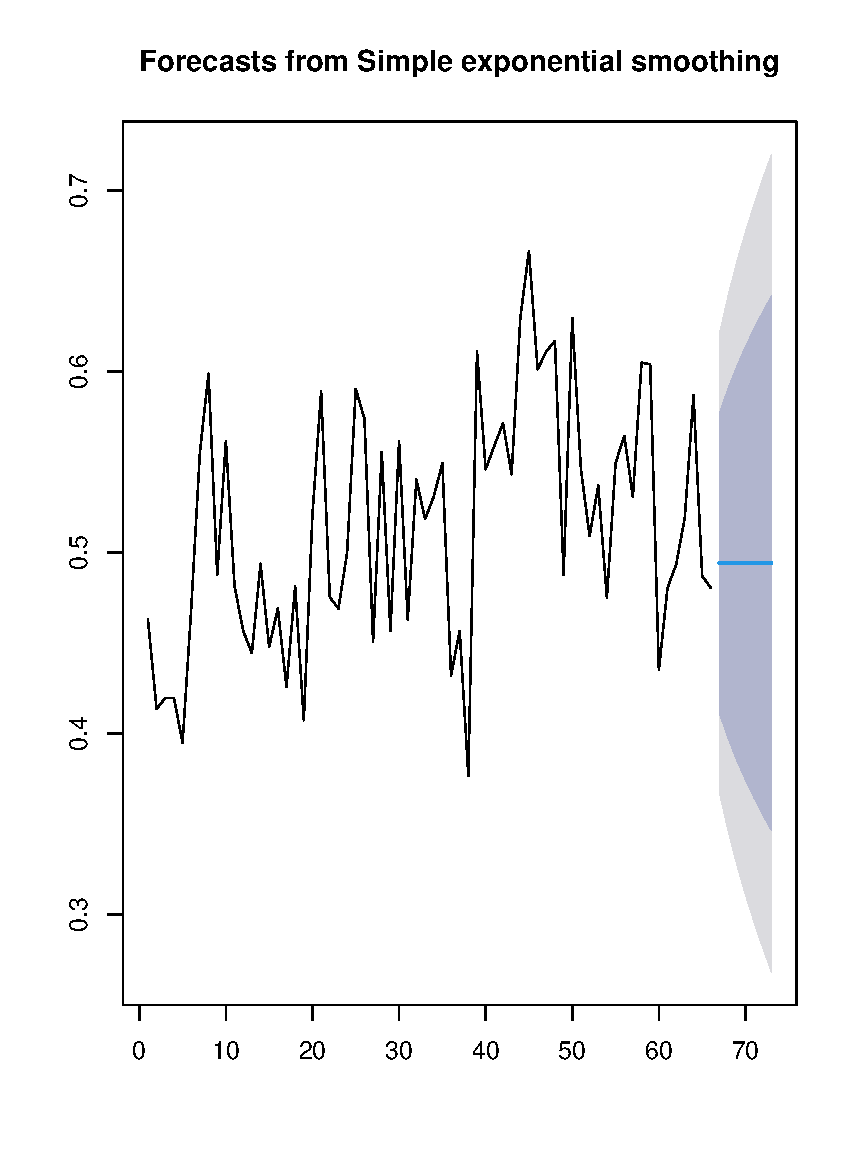
\includegraphics[width=0.9\linewidth, height=9cm]{es fore.pdf}
\caption{ES Forecast}
\label{fig:subim2}
\end{subfigure}
\begin{subfigure}{0.32\textwidth}
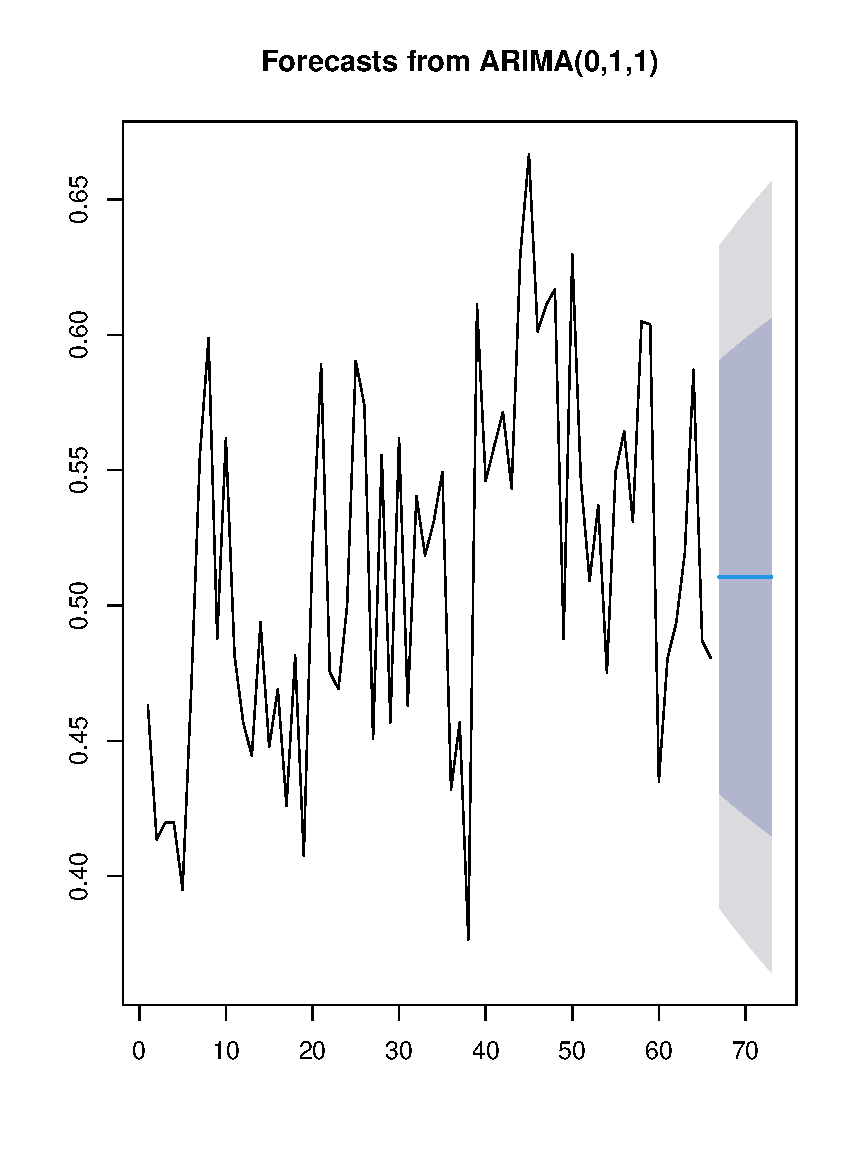
\includegraphics[width=0.9\linewidth, height=9cm]{arima fore.pdf} 
\caption{ARIMA(0, 1, 1) Forecast}
\label{fig:subim3}
\end{subfigure}
\caption{Forecast Plots}
\label{fig:Figure 5}
\end{figure}\\
\newpage
\section{Model Selection and Conclusion}\label{sec:chapter}
Table 2 gives the RMSE, MAE, and MAPE of each model's forecasts:
\begin{table}[h]
\begin{center}
\begin{tabular}{ |c|c|c|c| } 
 \hline
 \textbf{Model/Method} & \textbf{RMSE} & \textbf{MAE} & \textbf{MAPE}\\
 \hline
 Holt-Winters & 0.1985 & 0.0435 & 10.1915\\
 \hline
 ARIMA(0, 1, 1) & 0.2743 & 0.0753 & 17.5979\\ 
 \hline
 Exp. Smoothing & 0.2426 & 0.0588 & 13.8162\\ 
 \hline
\end{tabular}
\caption{Accuracy of Our Forecasts}
\label{table:Table 2}
\end{center}
\end{table}\\
From this table, we can see that the Holt-Winters model has the smallest error values across all 3 measures, indicating it is the best of the three methods at modeling a team's year-by-year winning percentage. When I look at these results, it makes sense that a model that assumes a nonconstant mean is the most effective model. In the context of our data, winning percentages for teams change, not only by year, but by every few years, as it is common to see teams struggle for multiple years and succeed for multiple years. It is not accurate to think that the only deviations from the average winning percentage for a given team are due to variance and not a trend.\\
When it comes to the question of whether a model of this type (Holt-Winters) will be accurate at modeling and forecasting other teams' winning percentages, I tend to think it will, as the inherent logic behind the model is accurate for most teams; there are trends to a team's winning percentage that can be predicted, and the average winning percentage of the team is a good place to start, and once the model recognizes the trend of a certain team, it can become extremely effective at predicting when success will start after a prolonged period of failure and vice-versa.\\

\section{References}\label{sec:chapter}
[1] https://www.baseball-reference.com/teams/CIN/index.shtml
\end{document}